\section{Auswertung} % (fold)
\label{sec:auswertung}

Alle Fehlerrechnungen wurden mithilfe Gaußscher Fehlerfortpflanzung errechnet.
\begin{equation}
	\Delta f(x_\text{1}\text{,...,}x_\text{n}) = \sqrt{\sum_\text{i=0}^\text{n} \left(\frac{\partial f}{\partial x_\text{i}} \Delta x_\text{i}\right)^2}
\end{equation}
Dafür ist die Python Bibliothek \textit{uncertainties} benutzt worden.

Wenn nicht anders angegeben gelten die Fehler
\begin{eqnarray}
	\Delta \SI{}{\volt} &=& \pm 5 ,\\
	\Delta \SI{}{\hertz} &=& \pm 0.5 ,\\
	\Delta \SI{}{\milli\meter} &=& \pm 0.005 ,\\
	\Delta \SI{}{\decibel} &=& \pm 0.5 .\\
\end{eqnarray}

\subsection{Untersuchung eines Reflexklystrons} % (fold)
\label{sub:untersuchung_der_}

\begin{figure}
	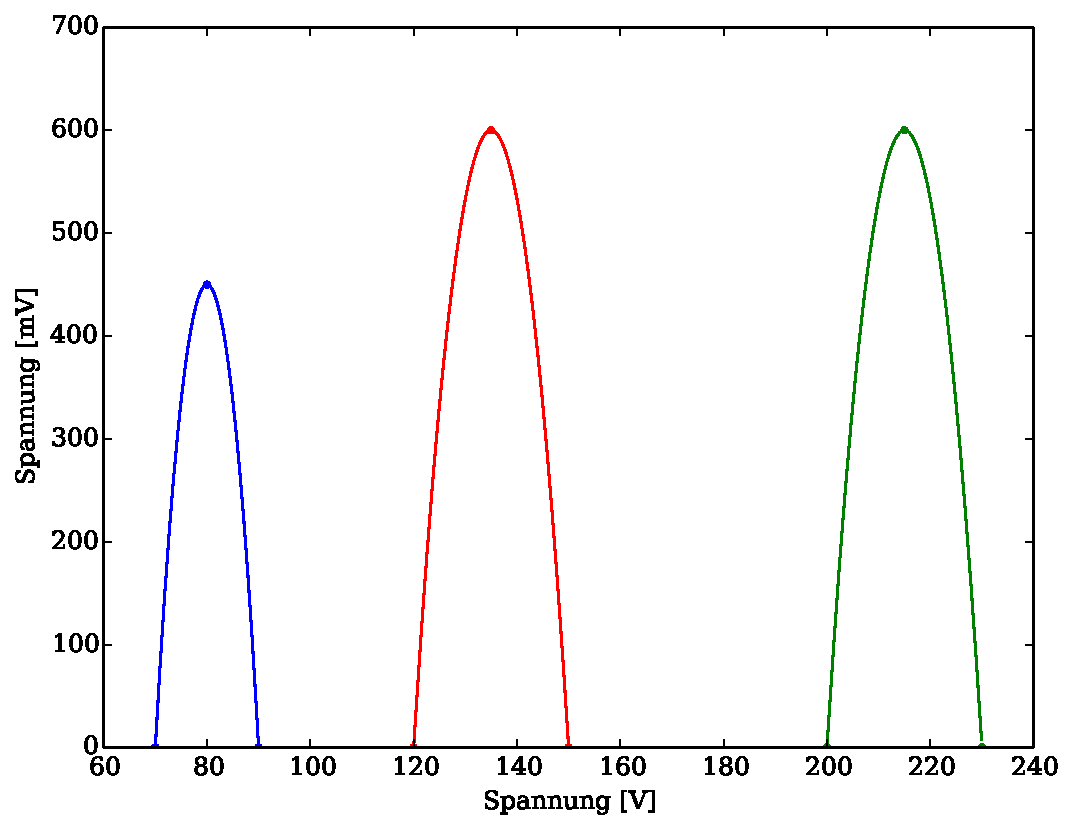
\includegraphics[width = 14cm]{pic/ModenDiagramm.pdf}
	\caption[]{Modus-Diagramm des Reflexklystrons bei einer Abstimmung auf $\SI{9}{\giga\hertz}$. Die Leistung der Amplitude ist proportional zur Spannung.}
	\label{mode}
\end{figure}

Nach der Abstimmung des Klystrons auf $\SI{9}{\giga\hertz}$ und der Bestimmung der Modenbreiten und Amplituden, hat sich das in Abbildung \ref{mode} dargestellte Modus-Diagramm ergeben.
Zur Darstellung wurde eine Parabelfunktion durch die Messpunkte gelegt.
Für die Abstimm-Empfindlichkeit $B$ des Klystrons hat sich nach Gleichung \eqref{eqn:empfindlichkeit}
\begin{eqnarray}
	%B &=& \frac{f'-f''}{V'-V''}\\
	B &=& \SI{2.1(7)}{\hertz\per\volt}
\end{eqnarray}
ergeben.

Die benutzten Daten sind in den Tabellen \ref{v1:1} und \ref{v1:2} aufgelistet.

\begin{table}
\centering
\caption{Messwerte zur Darstellung des Modus-Diagramms.}
\begin{tabular}{r r r r r r}
	Mode & $V_\text{0}[\SI{}{\volt}]$ & $V_\text{1}[\SI{}{\volt}]$ & $V_\text{2}[\SI{}{\volt}]$ & $A_\text{0}[\SI{}{\milli\volt}]$ & $f[\SI{}{\mega\hertz}]$ \\
	\hline
	\hline
	1 & 215 & 200 & 230 & {600(10)} & 9000.5\\
	2 & 185 & 120 & 150 & {600(10)} & 9005.0\\
	3 &  80 &  70 &  90 & {450(10)} & 9010.5\\
	\hline
\end{tabular}
\label{v1:1}
\caption{Messwerte zur Bestimmung der Banbreite $B$ des Klystrons.}
\begin{tabular}{r r r r r r}
	$V_\text{0}[\SI{}{\volt}]$ & $V'[\SI{}{\volt}]$ & $V''[\SI{}{\volt}]$ & $f_\text{0}[\SI{}{\mega\hertz}]$  & $f'[\SI{}{\mega\hertz}]$ & $f''[\SI{}{\mega\hertz}]$ \\
	\hline
	\hline
	215 & 225 & 205 & 9001.0 & 9024.0 & 8982.5\\
	\hline
\end{tabular}
\label{v1:2}
\end{table}

\FloatBarrier

\subsection{Messung von Frequenz, Wellenlänge und Dämpfung} % (fold)
\label{sub:messung_von_frequenz_wellenlaenge_und_daempfung}

\begin{figure}
	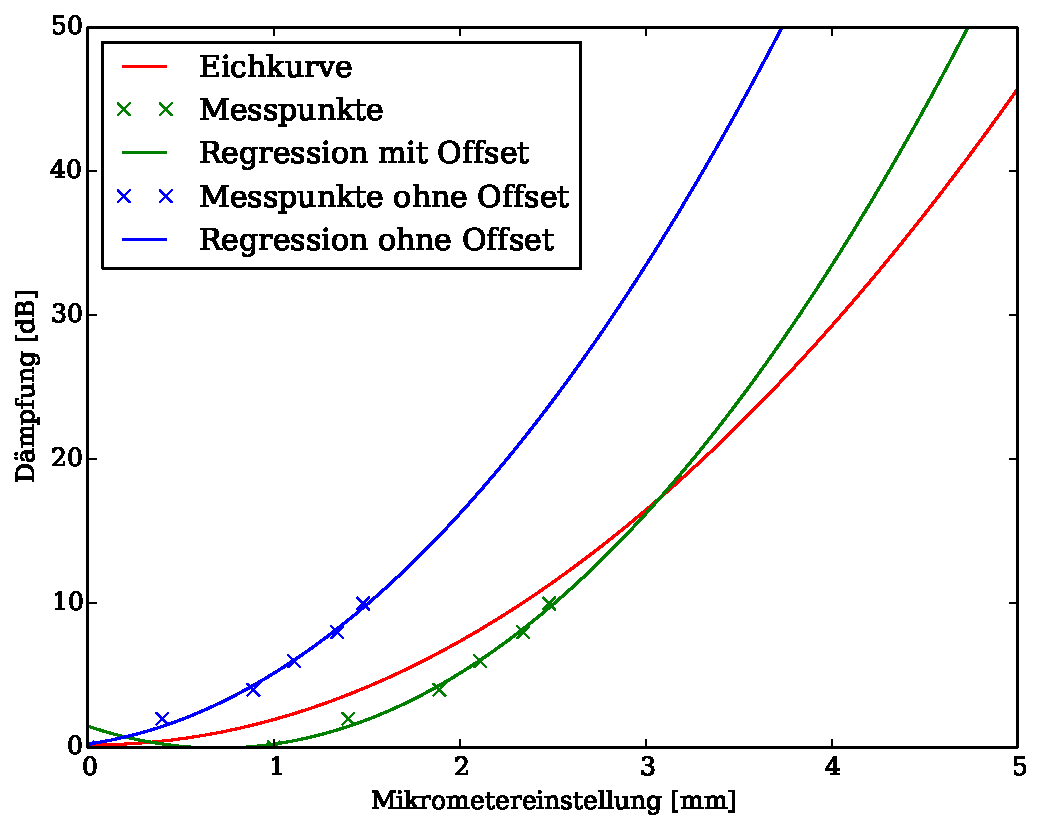
\includegraphics[width = 14cm]{pic/Daempfung.pdf}
	\caption[]{Dämpfungskurven des Klystrons.}
	\label{daempf}
\end{figure}

Die Bestimmung der Wellenlänge aus dem doppelten Abstand zweier Minima und der Frequenz nach Gleichung \eqref{frequenz} hat
\begin{eqnarray}
	\lambda &=& \SI{48.933(5)}{\milli\meter},\\
	f &=& \SI{8974(10)}{\mega\hertz}
\end{eqnarray}
ergeben.
Um die Wellenlänge zu bestimmen, wurde zunächst der Abstand zweier benachbarter Minima errechnet und anschließend über alle Abstände gemittelt (Vgl. Werte Tabelle \ref{v2:1}).
Es ist zu erkennen, dass die errechnete Frequenz des Klystrons der nahe kommt, auf welche das Klystron zuvor eingestellt worden ist.\\

Die Bestimmung der Dämpfungskurve mithilfe des SWR-Meters und dem Dämpfungsgliedes ergiebt die in Abbildung \ref{daempf} dargestellte Kurve.
Die verwendeten Werte sind in Tabelle \ref{v2:2} angegeben.
Diese wurde mit der Funktion
\begin{equation}
	f(x)=a \cdot (x-d)^2 + b \cdot (x-e) + c
\end{equation}
durch eine nicht linearen Regression erzeugt.
Die Fitparameter sind in Tabelle \ref{v2:3} dargestellt.

Es ist zu erkennen, dass die Dämpfungskurve steiler ansteigt als die Eichkurve der Dämpfungsgliedes.

\begin{table}
\centering
\caption{Messwerte zur Bestimmung der Klystronfrequenz.}
\begin{tabular}{r r r r r r}
	$f_\text{0}[\SI{}{\mega\hertz}]$ & $d_\text{1}[\SI{}{\milli\meter}]$ & $d_\text{2}[\SI{}{\milli\meter}]$ & $d_\text{3}[\SI{}{\milli\meter}]$ & $d_\text{4}[\SI{}{\milli\meter}]$ & $a[\SI{}{\milli\meter}]$\\
	\hline
	\hline
	8996.0 & 114.2 & 89.6 & 65.0 & 40.8 & $\SI{22.860(46)}{}$\\
	\hline
\end{tabular}
\label{v2:1}
\caption{Messwerte zur Bestimmung Dämpfungskurve.}
\begin{tabular}{r|r r r r r r|}
	SWR-Meter Ausschlag[$\SI{}{\decibel}$] & 0 & 2 & 4 & 6 & 8 & 10\\
	Mikrometereinstellung[$\SI{}{\milli\meter}$] & 1.00 & 1.40 & 1.89 & 2.11 & 2.34 & 2.48\\
\end{tabular}
\label{v2:2}
\caption{Fitparameter der Dämpfungskurven.}
\begin{tabular}{r r r r r r}
	 & a & b & c & d & e\\
	\hline
	\hline
	Regression m. Offset & 3.08 & 2.51 & 0.60 & 0.11 & 0.16\\
	Regression o. Offset & 3.08 & 1.00 & 0.60 & 0.86 & 1.42\\
	\hline
\end{tabular}
\label{v2:3}
\end{table}

\FloatBarrier

\subsection{Stehwellenmessungen VSWR} % (fold)
\label{sec:stehwellenmessungen_vswr}

Mithilfe der SWR-Meter Methode sind die in Tabelle \ref{v3:1} dargestellten SWR bei verschiedenen Sondentiefen ermittelt worden.\\

Mit der 3-dB-Methode bei einer Sodentiefe von $\SI{9}{\milli\meter}$ ergaben sich die Ergebnisse aus Tabelle \ref{v3:2}.
Das SWR wurde dabei nach der exakten Form der Gleichung \eqref{3dbswr} berechnet.\\

\begin{table}
	\centering
	\caption{Ergebnisse der SWR-Meter Methode.}
	\begin{tabular}{r || r r r r|}
	 Sondentiefe &    3 &    5 &    7 &    9\\
	        SWR & 1.20 & 1.55 & 3.00 & 6.00\\
	\end{tabular}
\caption{Ergebnisse der 3dB-SWR-Methode.}
	\label{v3:1}
	\begin{tabular}{r r r r r r r}
	$d_\text{1}[\SI{}{\milli\meter}]$ & $d_\text{2}[\SI{}{\milli\meter}]$ & $x_\text{min1}[\SI{}{\milli\meter}]$ & $x_\text{min2}[\SI{}{\milli\meter}]$ & $x_\text{min3}[\SI{}{\milli\meter}]$ & $\lambda[\SI{}{\milli\meter}]$ & SWR\\
	\hline
	\hline
	96.4 & 93.4 & 90.5 & 66.0 & 115.3 & $\SI{49.300(7)}{}$ & $\SI{5.357(12)}{}$\\
	\end{tabular}
	\caption{Ergebnisse der Abschwächer-Methode.}
	\label{v3:2}
	\begin{tabular}{r r r r}
	$A_\text{1}[\SI{}{\decibel}]$ & $A_\text{2}[\SI{}{\decibel}]$ & $A_\text{2}-A_\text{1}[\SI{}{\decibel}]$ & SWR\\
	\hline
	\hline
	20 & 40 & $\SI{20.0(7)}{}$ & $\SI{10.0(8)}{}$\\
	\end{tabular}
	\label{v3:3}
\end{table}

Mit der Abschwächer-Methode bei einer Sondentiefe von $\SI{9}{\milli\meter}$ ergaben sich die Ergebnisse aus Tabelle \ref{v3:3}.\\


\section{Diskussion} % (fold)
\label{sec:diskussion}

Bei der Untersuchung des Reflexklystrons stellte sich heraus, dass es gut möglich ist mit diesem ein Modus-Diagramm zu erzeugen.\\

Die errechnete Frequenz von $\SI{8974(10)}{\mega\hertz}$ liegt zudem nah an der eingestellten Frequenz von $\SI{8996.0(5)}{\mega\hertz}$.
Beim Messen der effektiven Dämpfungskurve des Klystrons ergab sich eine steilere Kurve als die Eichkurve des Dämpfungsgliedes.
Dies könnte durch eine zusätzliche Dämpfung innerhalb der Geräte zustande kommen.\\

Für die Messung des SWR hat sich ergeben, dass die 3dB-SWR-Methode und die SWR-Meter Methode auf etwa dasselbe Ergebnis kamen.
Mithilfe der Abschwächer-Methode hingegen ergab sich etwa der doppelte Wert.
Da die Sondentiefe mit $\SI{9}{\milli\meter}$ relativ groß ist, sollte die SWR-Meter Methode nicht hinreichend sein, da es zu Feldverzerrungen kommen kann.
Am genauesten sollte die Abschwächer-Methode mit $SWR = \SI{10}{}$ sein, da diese die Abweichung des Detektors vom quadratischen Verhalten überwindet.\\

Abschließend lässt sich sagen, dass die Untersuchung von Mikrowellen mit dem Reflexklystron hinreichend genau sind.
